\documentclass[11pt]{article}
\usepackage[T1]{fontenc}
\usepackage[utf8]{inputenc}
\usepackage{lmodern,amsmath,amssymb,graphicx,booktabs,tabularx,array,microtype,flafter,placeins,float}
\usepackage[margin=1in]{geometry}
\usepackage[colorlinks=true,linkcolor=black,citecolor=black,urlcolor=blue]{hyperref}
\setlength{\emergencystretch}{2em}
\title{When Compressed CRPS Depends on Measurement Units:\\Diagnosis and an Affine-Stable Correction}
\author{Hurcheson Asante Ofori and Jeffery Opoku}
\date{}

\begin{document}
\maketitle

\begin{abstract}
The continuous ranked probability score, or CRPS, is used to judge probability forecasts. We audit public code released with a kernel quadrature paper. Its compressed routine applies an equal-weight correction to unequal weights. We derive the resulting translation error and verify the formula against unchanged code. We then give an affine-standardized weighted CRPS wrapper. The wrapper standardizes an ensemble before compression and maps the score back to the original units. We prove that its score has the correct behavior under every positive affine recoding. In controlled tests, 11 of 12 settings pass the planned numerical checks; the failed setting remains a failure. We also study 39,575 temperature cases and 2,749 precipitation cases. Celsius-to-Kelvin conversion changes every released temperature score. For precipitation, millimetre-to-inch conversion gives a maximum released-score error of 14.90 mm after conversion back to the original units. A stricter affine recoding gives a median error of 34.00 mm. The affine-standardized wrapper stays within $4.46\times10^{-14}$ mm in both tests. Its median runtime is no larger than that of the released compressed routine in benchmarks with 100, 500, and 2,000 draws. However, an exact sorted fair CRPS is much faster in this univariate setting. The public repository still ends at its May 25, 2025 commit, which predates the final paper. Our claims therefore concern that public artifact, not a published figure. The wrapper is not a new proper score; it is a unit-stable way to run and score an unequal-weight compressor.
\end{abstract}

\section{Why this audit matters}

CRPS is widely used to compare probability forecasts. A lower score means that the forecast is closer to the observation while still giving a useful spread. Exact CRPS can be hard to compute, so researchers often estimate it from a finite set of forecast draws.

Different estimators answer different questions. The empirical CRPS scores the distribution made by the available draws. The fair CRPS estimates the population CRPS without the usual finite-ensemble bias when the draws are independent and identically distributed. A weighted empirical CRPS scores a distribution that puts different probabilities on different nodes. These targets are related, but they are not the same.

We study the public code linked to Adachi, Fujisawa, and Osborne \cite{adachi}. We use the repository at commit \texttt{dddd3ea46a6199d2ed48019c7825e79fb242787e}. The repository contains four commits, all dated May 25, 2025. A fresh remote check on October 10, 2026 found the same commit at the head of its only branch and found no later public release. The final paper appeared after that commit, and its compression equation uses an observation-dependent integrand that differs from the released compressor. We therefore define the object of study as the dated public artifact. We do not connect the affected path to a published figure.

This scope is intentional. The repository names the paper and contains the scoring and compression functions examined here. It does not contain the complete pipelines for the published convergence study, multisinusoidal comparison, or eight-dataset table. A defect in the released function is evidence about that implementation. It is not, by itself, evidence against every result in the paper.

We ask four questions.
\begin{enumerate}
\item Does the released code compute the same estimators that the paper describes?
\item Does the unequal weight correction preserve a basic property of CRPS when the measurement origin changes?
\item Does the issue survive full compression and change accuracy or model choice in controlled tests?
\item Can a simple wrapper restore the correct behavior under changes of both origin and scale without making the compressed routine slower?
\end{enumerate}

The paper does six things.
\begin{enumerate}
\item It separates the equation in the paper from the formula used in the released code.
\item It shows that the released uncompressed kernel routine matches the known fair CRPS on distinct samples.
\item It gives an exact formula for the translation error caused by using an equal weight correction with unequal weights.
\item It gives and proves an affine-standardized weighted CRPS wrapper for unequal-weight compression.
\item It reports full workflow tests on synthetic, temperature, and precipitation forecasts, including a failed planned check and a claim that did not transfer to the released code.
\item It compares runtime and accuracy against both pairwise and sorted exact fair CRPS.
\end{enumerate}

The fair CRPS and weighted empirical CRPS are not new. They come from earlier work on scoring rules and ensemble evaluation \cite{matheson,gneiting,ferro,zamo,bouallegue,kelen}. Positive weighted kernel quadrature is also established \cite{hayakawa}. Our contribution is narrower. We give the source-specific identity, check it against unchanged code, and measure its effect. We also give a general affine-standardization wrapper with an exact transformation law. The wrapper does not change the underlying score. It controls what numerical object reaches the compressor.

This matters in practice. A translation changes the zero point of a measurement, not the forecast error. A positive scale change changes only the unit size. Temperatures in Celsius and Kelvin test the first case. Precipitation in millimetres and inches tests the second. A CRPS implementation should transform predictably under both changes. It should not change a model ranking only because the same physical forecast is written in another unit system.

\subsection*{Source-to-paper map}

Table~\ref{tab:mapping} records what can and cannot be linked. This keeps a source-code result from being presented as a reproduction of an experiment whose full pipeline was not recovered.

\begin{table}[htbp]
\centering
\caption{Mapping between the final paper and the pinned public repository. ``Mapped'' means that the mathematical object is identifiable, not that a published experiment was reproduced.}
\label{tab:mapping}
\small
\begin{tabularx}{\textwidth}{>{\raggedright\arraybackslash}p{0.21\textwidth}>{\raggedright\arraybackslash}p{0.27\textwidth}X}
\toprule
Object & Released evidence & Audit status \\
\midrule
Analytical CRPS & \texttt{utils/crps.py}, \texttt{exact\_crps} & Mapped up to an equivalent sign convention \\
Right-ECDF PWM & \texttt{pwm\_function\_sample} & Different finite-sample formula because source ranks start at zero \\
Strict pair kernel & \texttt{indicator\_kernel} & Mapped for distinct samples \\
Uncompressed score & \texttt{error\_terms\_kq\_non\_comp} & Equals the historical fair CRPS on distinct draws \\
Compression target & \texttt{kq\_compress} receives the pair kernel alone & Does not match the final paper's observation-dependent full integrand \\
Compressed correction & \texttt{error\_terms\_kq\_comp} & Uses $m/(m-1)$ with unequal weights; defect verified \\
Published figures and tables & No complete matching pipelines or configurations in the pinned tree & Not reproduced and not challenged here \\
Repository status & Remote branch and commit history checked on October 10, 2026 & Public head remains the May 25, 2025 commit used in this audit \\
\bottomrule
\end{tabularx}
\end{table}

\section{The score formulas}

Let $x_1,\ldots,x_M$ be forecast draws and let $y$ be the observation. Define
\[
A=\frac{1}{M}\sum_{i=1}^M |x_i-y|,
\qquad
\bar{x}=\frac{1}{M}\sum_{i=1}^M x_i.
\]
The empirical CRPS is
\[
S_{\mathrm{emp}}=A-\frac{1}{2M^2}\sum_{i,j=1}^M |x_i-x_j|.
\]
The fair CRPS is
\[
S_{\mathrm{fair}}=A-\frac{1}{2M(M-1)}\sum_{i,j=1}^M |x_i-x_j|.
\]
For independent draws from the forecast distribution, $S_{\mathrm{fair}}$ is an unbiased estimate of the population CRPS \cite{ferro,zamo}.

For distinct draws, the equation based on the right empirical distribution function in the target paper gives
\[
S_{\mathrm{right}}=S_{\mathrm{emp}}-\frac{\bar{x}}{M}.
\]
The released function \texttt{pwm\_function\_sample} uses zero based ranks and gives
\[
S_{\mathrm{source}}=S_{\mathrm{emp}}+\frac{\bar{x}}{M}.
\]
The two formulas differ by $2\bar{x}/M$. A common shift of the forecast and observation changes them by opposite amounts. This difference matters when models use different ensemble sizes or when another part of the method makes the offset model dependent.

The released uncompressed kernel routine uses the factor $M/(M-1)$ with a zero diagonal pair average. On distinct samples, it equals $S_{\mathrm{fair}}$. This identity is known. Our tests only confirm how the released code behaves.

\begin{table}[htbp]
\centering
\caption{The estimators answer different questions. None should be called a general replacement for the others.}
\small
\begin{tabularx}{\textwidth}{>{\raggedright\arraybackslash}p{0.20\textwidth}X>{\raggedright\arraybackslash}p{0.23\textwidth}}
\toprule
Method & What it scores or estimates & Main condition \\
\midrule
Empirical CRPS & The empirical distribution formed by the available draws & No population unbiasedness claim \\
Fair CRPS & The population CRPS from independent and identically distributed draws & Exchangeable draws and $M\geq2$ \\
Released PWM & The source formula $S_{\mathrm{emp}}+\bar{x}/M$ & Distinct draws for the stated identity \\
Normalized pair score & A fixed weight algebraic correction & Distinct nodes and fixed weights \\
Weighted empirical CRPS & The discrete distribution with normalized node weights & Scores the compressed distribution \\
ASW-CRPS & Weighted empirical CRPS after location and range standardization & Affine-stable wrapper; no population unbiasedness claim \\
\bottomrule
\end{tabularx}
\end{table}

\section{Main mathematical result}

The compressed routine returns nodes $z_1,\ldots,z_m$ and nonnegative weights $w_1,\ldots,w_m$. The weights are usually unequal. For $i\ne j$, define
\[
h_{ij}=\frac{1}{2}\max(z_i,z_j),
\qquad h_{ii}=0.
\]
The released score has the form
\[
R(z,y)=\sum_i w_i|z_i-y|+\sum_i w_i z_i
-2k\sum_{i,j}w_iw_jh_{ij},
\qquad k=\frac{m}{m-1}.
\]

\subsection*{Proposition}
Suppose the nodes are distinct and the weights stay fixed. Let
\[
s=\sum_i w_i,
\qquad q=\sum_i w_i^2.
\]
If every node and the observation are shifted by the same number $c$, then
\[
R(z+c,y+c)-R(z,y)=c\{s-k(s^2-q)\}.
\]
If the weights sum to one, this becomes
\[
R(z+c,y+c)-R(z,y)
=c\frac{mq-1}{m-1}.
\]
The change is zero for uniform weights. It is usually not zero for unequal weights.

\subsection*{Proof}
The absolute error term does not change because
$|(z_i+c)-(y+c)|=|z_i-y|$. The weighted mean increases by $cs$. For $i\ne j$, the pair function increases by $c/2$. Its diagonal stays zero. The total off diagonal weight is
\[
\sum_{i\ne j}w_iw_j=s^2-q.
\]
The pair term therefore changes by $-ck(s^2-q)$. Adding this to the change $cs$ in the mean term gives the first formula. Setting $s=1$ and $k=m/(m-1)$ gives the second formula. \hfill$\square$

This proposition is about fixed nodes and fixed weights. It does not show that the whole compression process is translation invariant. It also does not show that a corrected score is unbiased after the nodes and weights are chosen from the data.

If float32 arithmetic makes two nodes equal after a shift, the distinct node assumption fails. One such case occurred in our tests. This is a real numerical boundary, not a reason to discard the failed check.

\subsection*{What the proposition settles}
The proposition gives a direct check for the released score. If the weights are unequal, the score has a nonzero translation term before compression is run again. This result does not depend on a simulation, a forecast family, or a chosen observation. It also explains why replacing $m/(m-1)$ with $1/(1-q)$ repairs the fixed-weight identity. That replacement does not answer the harder question: what happens when the nodes and weights are selected from the same sample.

\section{An affine-standardized compression wrapper}

The previous result diagnoses one formula. We now give a wrapper that can be used with any one-dimensional compressor. It handles changes in both the zero point and the unit size.

Let $x=(x_1,\ldots,x_M)$ be an ensemble. Define
\[
\ell(x)=\min_i x_i,
\qquad
r(x)=\max_i x_i-\min_i x_i.
\]
When $r(x)>0$, standardize the ensemble and observation as
\[
u_i=\frac{x_i-\ell(x)}{r(x)},
\qquad
v=\frac{y-\ell(x)}{r(x)}.
\]
Run the compressor on $u$ with a fixed random seed. Let its returned nodes and normalized weights be $z_1,\ldots,z_m$ and $p_1,\ldots,p_m$. We define the affine-standardized weighted score, or ASW-CRPS, by
\[
S_{\mathrm{ASW}}(x,y)
=r(x)\left\{
\sum_i p_i|z_i-v|
-\frac12\sum_{i,j}p_ip_j|z_i-z_j|
\right\}.
\]
If $r(x)=0$, we set $S_{\mathrm{ASW}}(x,y)=|x_1-y|$. This is the exact CRPS of a point mass.

\subsection*{Affine transformation proposition}
Suppose the same deterministic compressor and random seed are used in both unit systems. For $a>0$ and $b\in\mathbb{R}$, let $x'=ax+b$ and $y'=ay+b$. Then
\[
S_{\mathrm{ASW}}(x',y')=aS_{\mathrm{ASW}}(x,y).
\]
Therefore a positive affine change of units cannot change a model ranking based on ASW-CRPS.

\subsection*{Proof}
The transformed location and range are
\[
\ell(x')=a\ell(x)+b,
\qquad
r(x')=ar(x).
\]
It follows that
\[
\frac{x'_i-\ell(x')}{r(x')}
=\frac{x_i-\ell(x)}{r(x)},
\qquad
\frac{y'-\ell(x')}{r(x')}
=\frac{y-\ell(x)}{r(x)}.
\]
The compressor therefore receives the same standardized values and returns the same nodes and weights. The weighted score inside braces is unchanged, while the outside range is multiplied by $a$. This proves the result. The constant-ensemble case follows directly from $|ax_1+b-(ay+b)|=a|x_1-y|$. \hfill$\square$

The implementation rounds standardized coordinates to six decimal places before converting them to the float32 input used by the released compressor. This fixed numerical grid prevents two mathematically equal standardized inputs from landing on opposite sides of a float32 boundary. The rounding step is part of the implementation, not part of the theorem.

ASW-CRPS is not a new proper scoring rule. It applies the known weighted empirical CRPS after a deterministic change of coordinates. It guarantees the right transformation law, but it does not make adaptively selected nodes unbiased for population CRPS.

\section{Study design and decision rules}

All comparisons are paired. Methods use the same observations and forecast draws. A translated pair uses the same compression seed. Smaller ensemble sizes use prefixes of the same 500 draws. These choices remove avoidable Monte Carlo differences between methods and computing budgets.

Accuracy is measured against conditional population CRPS. Closed forms are used where available. Independent numerical integration checks the reference calculations. RMSE intervals use 2,000 bootstrap samples. The bootstrap resamples the 50 independent datasets as blocks, so it keeps all observations, candidates, methods, and origins from a dataset together. The intervals are cell level intervals. They are not simultaneous intervals over the whole study.

The main robustness rule was fixed before the run. All 12 cells had to pass their controls. At least 10 cells had to exceed the original median shift threshold of 0.01, with at least three cells in each family. A correction passed a cell only if its RMSE was lower than the original at both origins and both upper confidence limits were below zero. We report the failed global rule without changing its threshold.

The four forecast candidates are $(0,1)$, $(0,0.9)$, $(0.15,1)$, and $(0.15,0.9)$ in location and scale. This grid is small and one-sided. The model-choice results are therefore diagnostic. They do not estimate performance over all forecasting problems.

The affine extension uses 2,749 precipitation cases with 11 ensemble members. It tests a millimetre-to-inch conversion and a positive affine recoding $x'=x/25.4+10$. Scores from the transformed system are mapped back to millimetres before comparison. The planned numerical tolerance is $2\times10^{-4}$ mm. The runtime study uses standard Normal ensembles with 100, 500, and 2,000 draws. Each cell has 12 independent repetitions. It compares the released compressed score, ASW-CRPS, pairwise fair CRPS, and the exact sorted fair CRPS formula.

\section{Tests on the released code}

\subsection{Uncompressed formulas}

We called the unchanged source functions on 180,000 Normal ensembles. The origins were 0, 1, and 10. The ensemble sizes were 20, 100, and 500. The largest difference between the released uncompressed kernel routine and an independent fair CRPS calculation was $8.89\times10^{-15}$. The largest absolute expectation check statistic was 1.132.

At origin 10 with $M=100$, the released PWM score averaged 0.33924803. The released kernel routine and the independent fair CRPS both averaged 0.23361075. The true CRPS was 0.23369498. These results agree with the formulas above.

\subsection{A claim that did not transfer}

An earlier experiment used the equation based score $S_{\mathrm{right}}$. It found a rise of 10.6 to 12.6 percentage points in wrong model selection. We repeated the design with the score used in the released code. The planned rule failed in all three tested families.

For the Normal family, the fair score selected the wrong model in 66.5 percent of datasets, while the released PWM score did so in 63.2 percent. For the lognormal family, the rates were 53.0 and 54.1 percent. For the Student $t$ family with 5 degrees of freedom, the rates were 64.7 and 63.2 percent. These results do not support a general claim that fair scoring always gives the lowest finite sample selection error.

\subsection{Fixed node test}

We tested 20 independent Normal ensembles with 200 draws, 100 landmarks, and 50 selected nodes. A common shift of 10 changed the released compressed score by values from 0.130163 to 0.495517. The median change was 0.334060. The mathematical formula above matched the observed changes. The largest error was $1.83\times10^{-6}$, below the planned tolerance of $2\times10^{-4}$. A uniform weight control changed by only $2.80\times10^{-6}$.

\subsection{Full compression test}

We next ran compression again after shifting the data. This test used 100 datasets. Each dataset had 10 Gaussian observations and four candidate forecasts. Each candidate had 200 draws. The original compressed method changed its selected forecast in 40 of 100 datasets.

The original method had RMSE values of 0.044322 at origin 0 and 0.184697 at origin 10. A normalized pair correction had RMSE values of 0.054249 and 0.048390. Weighted empirical CRPS had values of 0.043177 and 0.042926. Full fair CRPS had values of 0.042794 at both origins. The normalized pair correction fixed the fixed weight formula, but it made accuracy worse at origin 0.

\section{Robustness across distributions and budgets}

The main robustness study used centered unit variance Normal, lognormal, and Student $t$ distributions. It tested four computing settings: $(100,40,20)$, $(200,40,20)$, $(200,100,50)$, and $(500,100,50)$. These numbers give the ensemble size, landmark count, and requested node count. Each family had 50 independent datasets with 5 observations. Each dataset compared four forecast candidates.

The planned overall rule failed because one lognormal setting failed a numerical control. We did not change the rule after seeing the result. The other 11 settings passed all controls. In those 11 settings, the original method changed its selected forecast in 8 to 38 of 50 datasets. Weighted empirical CRPS changed its choice in 1 to 7 datasets. Full fair CRPS did not change its choice in any observed dataset.

Weighted empirical CRPS improved RMSE at both origins in 10 of the 11 valid settings. It failed the planned rule in the Student $t$ setting $(200,100,50)$ because the origin 0 confidence interval crossed zero. The estimated RMSE difference was $-0.000729$, with a 95 percent interval from $-0.001759$ to $0.000364$. The normalized pair correction passed in none of the 11 valid settings. Full fair CRPS passed against the original method in all 11 valid settings. We did not register a test claiming that weighted empirical CRPS beats full fair CRPS.

The failed lognormal setting was $(500,100,50)$. One float32 shift merged two nearby nodes. The smallest spacing was $5.960464477539063\times10^{-8}$. Shifting the same nodes after conversion to float64 reduced the errors to numerical roundoff. This explains the failure, but it does not make the planned result a pass.

\begin{figure}[htbp]
\centering
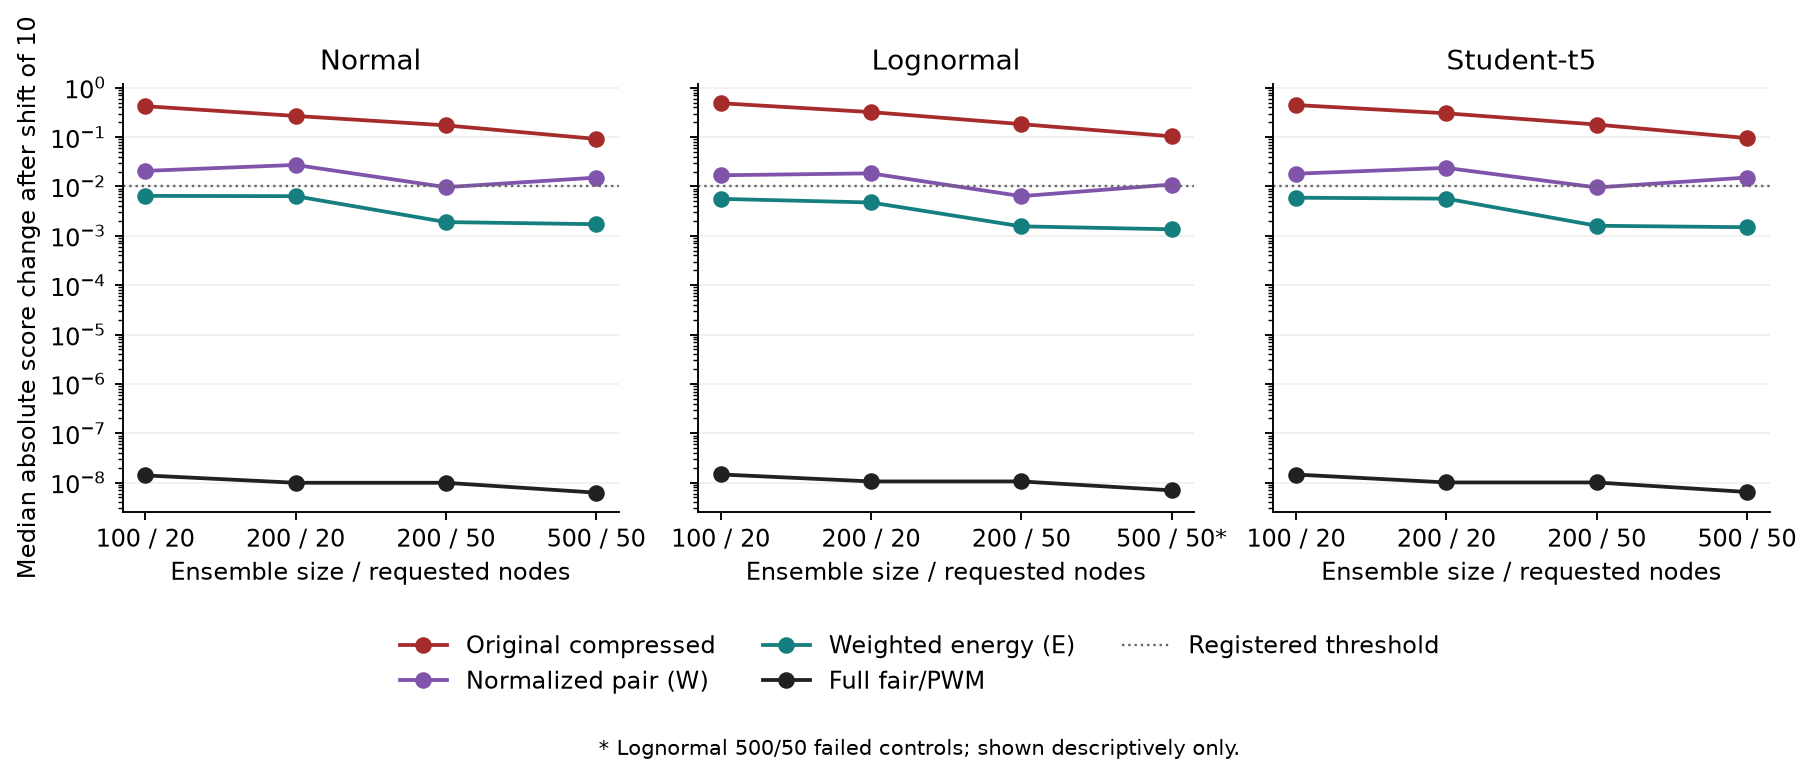
\includegraphics[width=\textwidth]{figures/origin.png}
\caption{Median score change after a common shift of 10. The asterisk marks the setting that failed a numerical control. That point is descriptive only.}
\end{figure}

\begin{figure}[H]
\centering
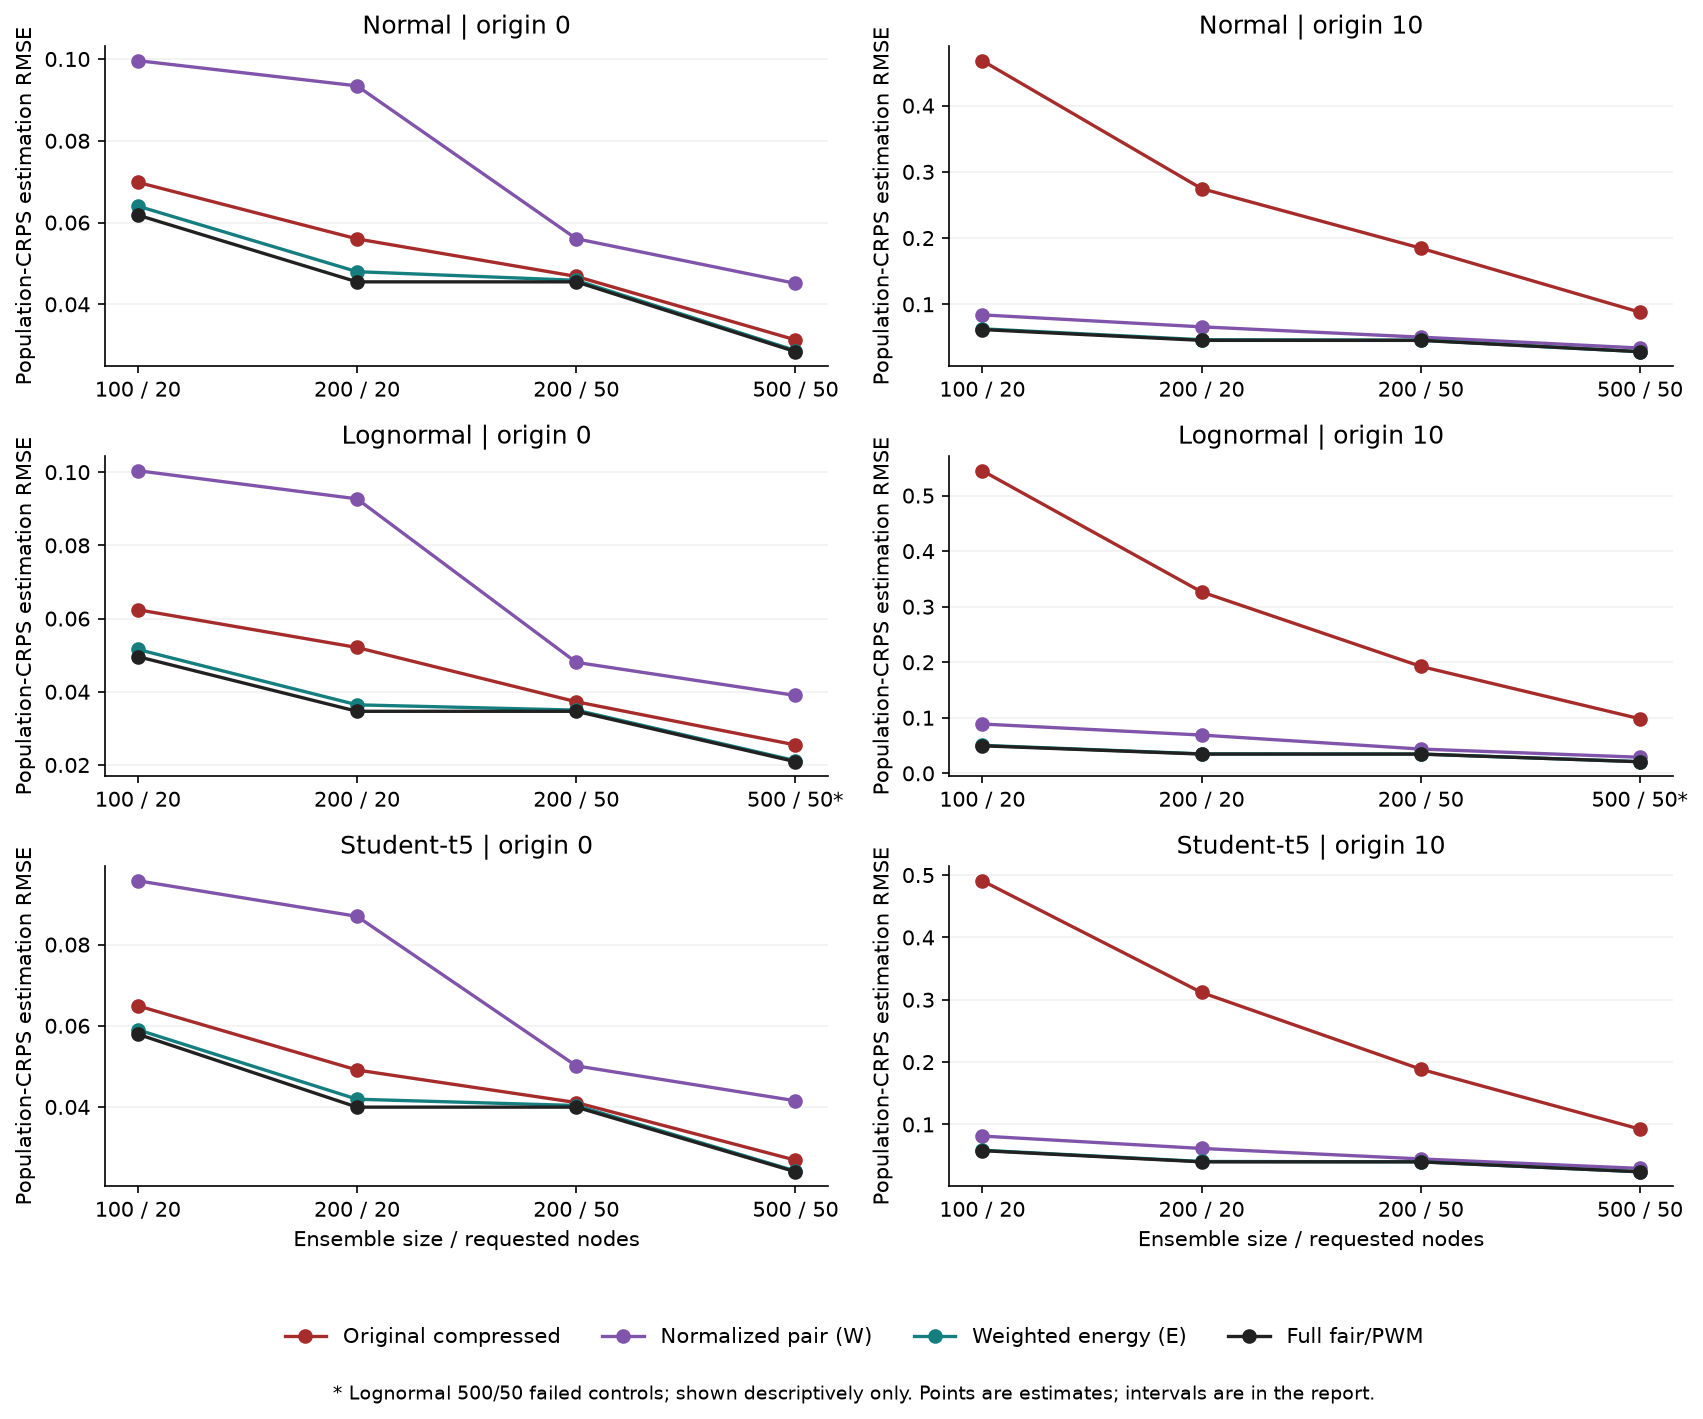
\includegraphics[width=0.82\textwidth]{figures/accuracy.png}
\caption{RMSE against population CRPS. The curves show point estimates. The report gives cell level confidence intervals.}
\end{figure}

\FloatBarrier

\section{What the results do and do not show}

\subsection{Real weather forecasts}

We preregistered the first real-data test before its first source-compression run. The data come from version 1.0-0 of the CRAN package \texttt{ensemblepp} \cite{ensemblepp}. They contain 2,749 observations of 12-hour minimum temperature at Innsbruck Airport and 11 corresponding 18--30 hour NOAA GEFS reforecast members. The cases run from January 2, 2000, through January 1, 2016. The source package has no missing values in these fields.

We then added a second real-data check using 36,826 Pacific Northwest surface-temperature forecasts from the same released data packet. These forecasts are stored in Kelvin. We repeated the same physical forecasts after subtracting 273.15, which writes them in Celsius. This second check used six landmarks and four compressed nodes. In both real-data checks, the released compressor remained in float32. Returned nodes and weights were scored in float64.

For Innsbruck, we used eight landmarks, five compressed nodes, and the same seed for both calls. For Pacific Northwest, we used six landmarks, four compressed nodes, and the same seed for both calls. All planned controls passed in both datasets. No source call failed. The largest weight-sum error was $2.91\times10^{-7}$ for Innsbruck and $5.33\times10^{-7}$ for Pacific Northwest. The full fair CRPS changed by at most $2.85\times10^{-14}$ degrees for Innsbruck and by exactly 0 in the Pacific Northwest run.

Table~\ref{tab:realdata} gives the primary result. The released compressed score changed by more than 0.01 degrees in every case in both datasets. Its median absolute change was 35.51 degrees for Innsbruck and 35.04 degrees for Pacific Northwest. Recompression also caused smaller changes in the normalized pair and weighted empirical scores because the selected nodes and weights can change after conversion. A translation-anchored weighted correction passed the strict invariance check in both real-data tests. Full fair CRPS also passed.

\begin{table}[htbp]
\centering
\caption{Absolute score change when the same forecasts are expressed in two temperature units. Innsbruck uses Celsius to Kelvin conversion. Pacific Northwest uses Kelvin to Celsius conversion. The practical pass rule requires a maximum no larger than $2\times10^{-4}$ degrees.}
\label{tab:realdata}
\small
\resizebox{\textwidth}{!}{%
\begin{tabular}{llrrrrc}
\toprule
Dataset & Method & Median & 95th percentile & Maximum & Above 0.01 & Pass \\
\midrule
Innsbruck & Released compressed & 35.508 & 86.717 & 152.811 & 2,749 & No \\
Innsbruck & Normalized pair & 0.041 & 0.448 & 6.576 & 2,202 & No \\
Innsbruck & Weighted empirical & 0.023 & 0.363 & 4.025 & 1,843 & No \\
Innsbruck & Anchored weighted & $1.15\times10^{-14}$ & $2.49\times10^{-14}$ & $3.02\times10^{-14}$ & 0 & Yes \\
Innsbruck & Full fair CRPS & $1.25\times10^{-14}$ & $2.49\times10^{-14}$ & $2.85\times10^{-14}$ & 0 & Yes \\
Pacific Northwest & Released compressed & 35.042 & 80.063 & 188.668 & 36,826 & No \\
Pacific Northwest & Normalized pair & 0.044 & 0.460 & 7.530 & 28,718 & No \\
Pacific Northwest & Weighted empirical & 0.026 & 0.349 & 4.843 & 25,466 & No \\
Pacific Northwest & Anchored weighted & 0 & 0 & 0 & 0 & Yes \\
Pacific Northwest & Full fair CRPS & 0 & 0 & 0 & 0 & Yes \\
\bottomrule
\end{tabular}
}
\end{table}

As a secondary check, we treated the full ensemble fair CRPS as the uncompressed reference. On 400 sampled rows with 10 seeds per row, the released compressed score had RMSE 1.648 for Innsbruck and 49.404 for Pacific Northwest. The anchored weighted correction had RMSE 0.106 and 0.126. Weighted empirical CRPS had RMSE 0.144 and 0.206. These values assess agreement with the uncompressed score, not forecast skill against an unknown population distribution.

We also ran a small rolling ranking study on the Innsbruck data. Four candidate forecasts were compared after a 365-case rolling history. The released compressed score changed the selected candidate after Celsius-to-Kelvin conversion in 1,624 of 2,384 cases, or 68.1 percent. Moving-block 95 percent intervals ranged from 66.1 to 70.1 percent across block lengths 7, 14, and 30. The anchored weighted correction and full fair CRPS changed no selected candidates.

\subsection{Precipitation and affine recoding}

Temperature changes between Celsius and Kelvin test a change of origin. We added 2,749 Innsbruck 12-hour precipitation forecasts to test a different variable and a change of scale. Each case has 11 ensemble members. Sixty-four ensembles are constant; ASW-CRPS handles them exactly as point masses.

Table~\ref{tab:precipitation} reports absolute score differences after mapping transformed scores back to millimetres. A millimetre-to-inch conversion changes only the unit size. The released compressed score has a small median difference, but its 95th percentile is 0.213 mm and its maximum is 14.90 mm. The stricter affine recoding $x'=x/25.4+10$ adds a change of origin. Under this recoding, the released score has a median difference of 34.00 mm and a maximum of 254.00 mm. ASW-CRPS and sorted fair CRPS remain at numerical roundoff in both tests. All planned controls pass.

\begin{table}[htbp]
\centering
\caption{Absolute score changes on 2,749 precipitation forecasts after transformed scores are returned to millimetres. The planned tolerance is $2\times10^{-4}$ mm.}
\label{tab:precipitation}
\small
\resizebox{\textwidth}{!}{%
\begin{tabular}{lrrrr}
\toprule
& \multicolumn{2}{c}{Millimetres to inches} & \multicolumn{2}{c}{Positive affine recoding} \\
Method & Median & Maximum & Median & Maximum \\
\midrule
Released compressed & $2.18\times10^{-6}$ & 14.898 & 34.000 & 254.000 \\
Weighted empirical & $3.31\times10^{-7}$ & 1.043 & 0.0156 & 3.651 \\
Translation anchored & $2.90\times10^{-7}$ & 0.695 & $2.90\times10^{-7}$ & 0.695 \\
ASW-CRPS & $2.78\times10^{-17}$ & $1.07\times10^{-14}$ & $8.10\times10^{-15}$ & $4.45\times10^{-14}$ \\
Sorted fair CRPS & $8.33\times10^{-17}$ & $1.07\times10^{-14}$ & $8.44\times10^{-15}$ & $4.62\times10^{-14}$ \\
\bottomrule
\end{tabular}
}
\end{table}

\FloatBarrier

\subsection{Runtime and accuracy}

ASW-CRPS keeps the runtime profile of the released compressor. Its median runtime is 14.16, 24.68, and 40.30 ms for ensemble sizes 100, 500, and 2,000. The released routine takes 14.74, 26.18, and 49.36 ms. Thus standardization does not make compression slower in these tests.

This result does not mean that compression is the fastest way to compute univariate CRPS. The exact sorted fair formula takes 0.106, 0.104, and 0.121 ms in the same cells. At 2,000 draws it is more than 300 times faster than ASW-CRPS. The direct pairwise fair calculation takes 0.058, 1.591, and 29.761 ms. The sorted formula avoids the quadratic pair matrix. Table~\ref{tab:runtime} therefore supports a limited conclusion: ASW-CRPS preserves the cost of the released compressed workflow, but exact sorted fair CRPS is the stronger practical baseline for one-dimensional ensembles.

\begin{table}[htbp]
\centering
\caption{Median runtime and RMSE against population CRPS for standard Normal draws. Each cell has 12 repetitions. Times are machine-specific and include compression when applicable.}
\label{tab:runtime}
\small
\begin{tabular}{rrrrrrr}
\toprule
$M$ & \multicolumn{2}{c}{Released compressed} & \multicolumn{2}{c}{ASW-CRPS} & \multicolumn{2}{c}{Sorted fair} \\
& ms & RMSE & ms & RMSE & ms & RMSE \\
\midrule
100  & 14.741 & 0.04539 & 14.155 & 0.03445 & 0.106 & 0.03587 \\
500  & 26.185 & 0.03665 & 24.677 & 0.00680 & 0.104 & 0.00832 \\
2000 & 49.361 & 0.02670 & 40.302 & 0.00897 & 0.121 & 0.00666 \\
\bottomrule
\end{tabular}
\end{table}

\FloatBarrier

The results support one clear conclusion. The released compressed routine applies an equal-weight correction to unequal weights. This creates a predictable translation error when nodes and weights are fixed. Running compression again can create a larger change because the selected nodes and weights can also change. Translation anchoring handles a change of origin, but it does not handle a change of scale. ASW-CRPS handles both changes in these tests and has the exact positive-affine law proved above. For a one-dimensional ensemble, the exact sorted fair CRPS is still the simpler and faster baseline when compression is not needed for another reason.

The results do not prove that a published figure is wrong. The released repository predates the final paper, and the final paper describes a different compression integrand. We have not recovered the exact code, data, checkpoints, and settings used for each published figure.

Weighted empirical CRPS is a useful comparison because it scores the compressed weighted distribution directly. It is not a new score. Translation anchoring and affine standardization are wrappers around the same score. The first subtracts a translation-invariant anchor. The second also divides by a positive scale and maps the result back to the original units. Neither wrapper proves population unbiasedness when nodes and weights are chosen adaptively. A method should state which distribution it scores before making a claim about bias.

The model-selection experiments are synthetic. Their forecast grid is small and uses only positive location errors. The main robustness study has five observations per dataset. The real-data checks add operational temperature and precipitation ensembles, but all three datasets are weather data. These choices make the paper a controlled software audit. They do not make it a broad test of forecasting practice.

A stronger external validation would add negative location errors, more scale errors, more locations, wind forecasts, and a non-weather domain. The present evidence is enough to test an implementation property because the affine transformation law is distribution free. It is not enough to estimate how often the defect changes decisions across all operational forecasting systems.

\subsection*{Threats to validity}

\textbf{Source mapping.} The public commit predates the final paper. The released compressor and the final paper use different integrands. This limits the claim to the released implementation.

\textbf{External validity.} The synthetic tests cover symmetry, skew, and heavy tails. The real-data checks add 39,575 temperature cases and 2,749 precipitation cases, for 42,324 cases in total. The cases come from two weather data sources. Other variables, regions, and ensemble systems may produce different magnitudes.

\textbf{Model grid.} The four candidates use only zero or positive location error. A symmetric grid could change finite sample selection rates. We therefore treat the ranking results as bounded evidence.

\textbf{Uncertainty.} The bootstrap has 50 independent blocks per cell. The intervals support cell level comparisons, not a claim that every result would repeat in a new study.

\textbf{Finite precision.} Compression uses float32 because the released code does. The one failed control shows that rounding can merge close nodes. The double precision replay explains the event but does not replace the planned result.

\subsection*{Practical correction path}

A safe software correction should start by naming the target. If the goal is to score the compressed discrete distribution, normalized weighted empirical CRPS is the direct choice. If only a common translation must be handled, the ensemble can first be shifted by a data-dependent anchor, such as its minimum member. If both origin and scale may change, ASW-CRPS is the stronger wrapper because it has an exact positive-affine transformation law. In the present benchmark it keeps the runtime of the released compressor. Still, exact sorted fair CRPS is much faster for a one-dimensional ensemble and should be the default when the full ensemble is available. If the goal is an unbiased estimate of population CRPS, adaptive node selection needs a separate proof. Changing only the pair correction to $1/(1-q)$ fixes the fixed-weight translation identity, but our tests show that it does not guarantee lower RMSE in the full workflow. Software should also promote returned nodes to float64 before score calculations and should test weight normalization, duplicate nodes, constant ensembles, translations, and changes of scale.

\section{Reproducibility}

The main robustness study uses Python 3.12.14, Torch 2.14.1 with CPU support, BoTorch 0.18.1, GPyTorch 1.15.2, NumPy 2.5.3, and SciPy 1.18.1. Its exact package set is stored in \texttt{requirements-main-lock.txt}. The expanded real-data and affine study uses Python 3.13.7, Torch 2.14.0 with CPU support, GPyTorch 1.15.2, NumPy 2.4.6, pandas 2.3.3, and SciPy 1.16.3. Its exact package set is stored in \texttt{requirements-real-data-lock.txt}. Compression remains in float32 because that is how the released source works. Score calculations use float64 after the source returns its nodes and weights.

The main robustness run completes 24,000 source compressions and 192 unchanged public score checks. The expanded validation adds 42,324 real forecast cases, seed and budget sensitivity checks, equal-budget comparisons, a rolling ranking study, precipitation affine tests, and runtime comparisons. The release includes the scripts, protocols, public data files, JSON results, tables, and figures needed to inspect these claims. It does not redistribute the upstream source tree. Instead, \texttt{real\_data/fetch\_pinned\_source.py} retrieves the named public commit and verifies its hash. \texttt{DATA\_SOURCES.md} records the origin of each included dataset.

A package-level script, \texttt{run\_all.py}, rebuilds the manuscript, runs unit tests for the affine wrapper, verifies the stored temperature and precipitation results, and writes \texttt{SHA256SUMS.txt}. The public package is at \href{https://github.com/jopoku16/crps-affine-audit}{github.com/jopoku16/crps-affine-audit}. The fixed release is archived at \href{https://doi.org/10.5281/zenodo.23288536}{doi:10.5281/zenodo.23288536}. \texttt{CITATION.cff} and \texttt{.zenodo.json} provide release metadata.

The documentary audit also records the source commit, a clean source diff, the publication PDF hash, the accessible repository history, and the exact objects used in the map in Table~\ref{tab:mapping}. The main simulation output stores per-case seeds, source-call diagnostics, support overlap, weight changes, score changes, reference values, and dataset-level error summaries. The failed cell and its later float64 diagnosis remain separate records. This keeps the planned verdict from being overwritten by a post-run explanation.

\section{Conclusion}

The released code contains a clear mismatch between unequal compression weights and an equal-weight correction. The resulting translation error has a simple exact formula. Direct calls to the unchanged code agree with that formula. Full-workflow tests show that the problem can change model rankings in the synthetic settings studied here. Temperature and precipitation data show that the problem is not tied to one variable or one kind of unit change.

ASW-CRPS gives a unit-stable way to keep the released compression workflow. Its exact positive-affine law is the main general result beyond the source audit. It is not a new proper score, and it does not prove unbiasedness after adaptive compression. For one-dimensional ensembles, exact sorted fair CRPS is both simpler and much faster in our benchmark. The paper therefore supports a precise correction and a practical diagnostic. It does not support a claim about every published experiment or every forecasting system.

\begin{thebibliography}{9}
\bibitem{matheson} J. E. Matheson and R. L. Winkler. Scoring Rules for Continuous Probability Distributions. \emph{Management Science}, 22(10):1087 to 1096, 1976. \href{https://doi.org/10.1287/mnsc.22.10.1087}{doi:10.1287/mnsc.22.10.1087}.
\bibitem{gneiting} T. Gneiting and A. E. Raftery. Strictly Proper Scoring Rules, Prediction, and Estimation. \emph{Journal of the American Statistical Association}, 102(477):359 to 378, 2007. \href{https://doi.org/10.1198/016214506000001437}{doi:10.1198/016214506000001437}.
\bibitem{ferro} C. A. T. Ferro. Fair scores for ensemble forecasts. \emph{Quarterly Journal of the Royal Meteorological Society}, 2014. \href{https://doi.org/10.1002/qj.2270}{doi:10.1002/qj.2270}.
\bibitem{zamo} M. Zamo and P. Naveau. Estimation of the Continuous Ranked Probability Score with Limited Information and Applications to Ensemble Weather Forecasts. \emph{Mathematical Geosciences}, 2018. \href{https://doi.org/10.1007/s11004-017-9709-7}{doi:10.1007/s11004-017-9709-7}.
\bibitem{adachi} M. Adachi, M. Fujisawa, and M. A. Osborne. Fixing the Pitfalls of Probabilistic Time Series Forecasting Evaluation by Kernel Quadrature. \emph{Proceedings of the First International Conference on Probabilistic Numerics}, PMLR 271:1 to 11, 2025. \href{https://proceedings.mlr.press/v271/adachi25a.html}{Publisher page}.
\bibitem{kelen} D. M. Kelen, A. Jung, P. Kersch, and A. A. Benczur. Distribution Free Data Uncertainty for Neural Network Regression. \emph{ICLR}, 2025. \href{https://proceedings.iclr.cc/paper_files/paper/2025/hash/3eceb70f47690051d6769739fbf6294b-Abstract-Conference.html}{Conference paper}.
\bibitem{bouallegue} Z. Ben Bouallegue, C. A. T. Ferro, M. Leutbecher, and D. S. Richardson. Predictive verification for the design of partially exchangeable multi model ensembles. \emph{Tellus A}, 72(1):1 to 12, 2020. \href{https://doi.org/10.1080/16000870.2019.1697165}{doi:10.1080/16000870.2019.1697165}.
\bibitem{hayakawa} S. Hayakawa, H. Oberhauser, and T. Lyons. Positively Weighted Kernel Quadrature via Subsampling. \emph{Advances in Neural Information Processing Systems}, 2022. \href{https://arxiv.org/abs/2107.09597}{arXiv:2107.09597}.
\bibitem{ensemblepp} J. W. Messner. \texttt{ensemblepp}: Ensemble Postprocessing Data Sets, version 1.0-0. CRAN, 2019. \href{https://cran.r-project.org/package=ensemblepp}{Package page}.
\end{thebibliography}

\medskip
\noindent\textsc{School of Mathematical and Statistical Sciences,
University of Texas Rio Grande Valley, Edinburg, Texas 78539, USA}

\noindent\emph{Email addresses:}
\texttt{hurcheson.ofori01@utrgv.edu},
\texttt{opokujeffery5@gmail.com}

\end{document}
